% ============================================================
%  Section 3: Method
%  AgentForge: A Multi-Agent Framework for Autonomous
%  Software Engineering
% ============================================================

\section{Method}
\label{sec:method}

We present \textbf{AgentForge}, a multi-agent framework for
autonomous software engineering. Given a natural language task
$\mathcal{T}$ and an optional set of context files
$\mathcal{F} = \{f_1, \dots, f_n\}$, AgentForge produces
verified, executable code $\hat{c}$ by routing the task through
a structured pipeline of five specialized agents, each
responsible for a single subtask.
Figure~\ref{fig:overview} shows the full system.

\begin{figure}[ht]
    \centering
    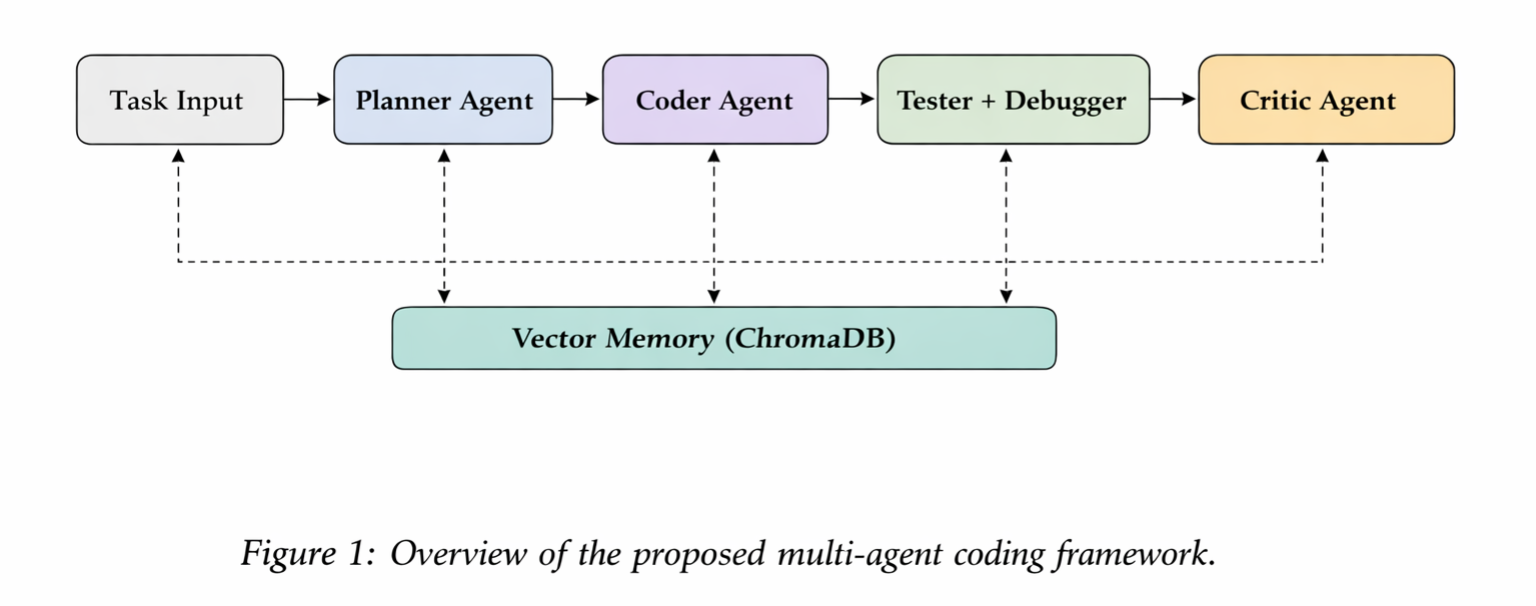
\includegraphics[width=\linewidth]{Figure2.png}
    \caption{Overview of the AgentForge multi-agent coding framework, illustrating the sequential handover between specialized agents and the shared Vector Memory.}
    \label{fig:overview}
\end{figure}

% ------------------------------------------------------------
\subsection{Problem Formulation}
\label{sec:formulation}

Let $\mathcal{T}$ be a natural language software engineering
task (e.g., \textit{``Add JWT authentication to the login
endpoint''}). Let $\mathcal{R}$ be a code repository and
$\mathcal{M}$ a memory store of previously solved tasks.
We seek a function $\Phi$ such that:

\begin{equation}
  \hat{c} = \Phi(\mathcal{T},\, \mathcal{R},\, \mathcal{M})
\end{equation}

\noindent where $\hat{c}$ is code that (i) satisfies
$\mathcal{T}$, (ii) passes automated tests in an isolated
execution environment, and (iii) receives a passing verdict
from an independent review agent. Unlike prior single-model
approaches~\cite{chen2021codex,li2022alphacode}, $\Phi$ is
realized as a coordinated pipeline of specialized agents
rather than a single forward pass.

% ------------------------------------------------------------
\subsection{System Overview}
\label{sec:overview}

AgentForge decomposes autonomous code generation into five
sequential roles: \textit{Planner}, \textit{Coder},
\textit{Tester}, \textit{Debugger}, and \textit{Critic}.
Each agent is implemented as a prompted large language model
(LLM) call with a role-specific system prompt. A central
\textit{Orchestrator} coordinates the pipeline, manages
shared memory, and handles the iterative debug loop.

\paragraph{Notation.}
Let $\mathcal{A} = \{A_\text{plan}, A_\text{code},
A_\text{test}, A_\text{debug}, A_\text{crit}\}$ denote the
agent set. Let $\pi_a$ denote the system prompt for agent
$a \in \mathcal{A}$, and let $\text{LLM}(\pi_a, x)$ denote
a call to the base language model with system prompt $\pi_a$
and user input $x$.

% ------------------------------------------------------------
\subsection{Memory and Context Retrieval}
\label{sec:memory}

Before planning, the Orchestrator enriches the task with
two sources of context: \textit{episodic memory} from past
tasks and \textit{semantic retrieval} from the live
repository index.

\paragraph{Episodic memory.}
Successful (task, code) pairs from prior runs are stored in
a persistent vector database (ChromaDB~\cite{chromadb}).
At inference time, the top-$k$ most similar past tasks are
retrieved by cosine similarity of their
\texttt{text-embedding-3-small} embeddings:

\begin{equation}
  \mathcal{M}_k = \underset{m \in \mathcal{M}}{\text{top-}k}
  \;\frac{\mathbf{e}_\mathcal{T} \cdot \mathbf{e}_m}
         {\|\mathbf{e}_\mathcal{T}\|\,\|\mathbf{e}_m\|}
\end{equation}

\begin{figure}[ht]
    \centering
    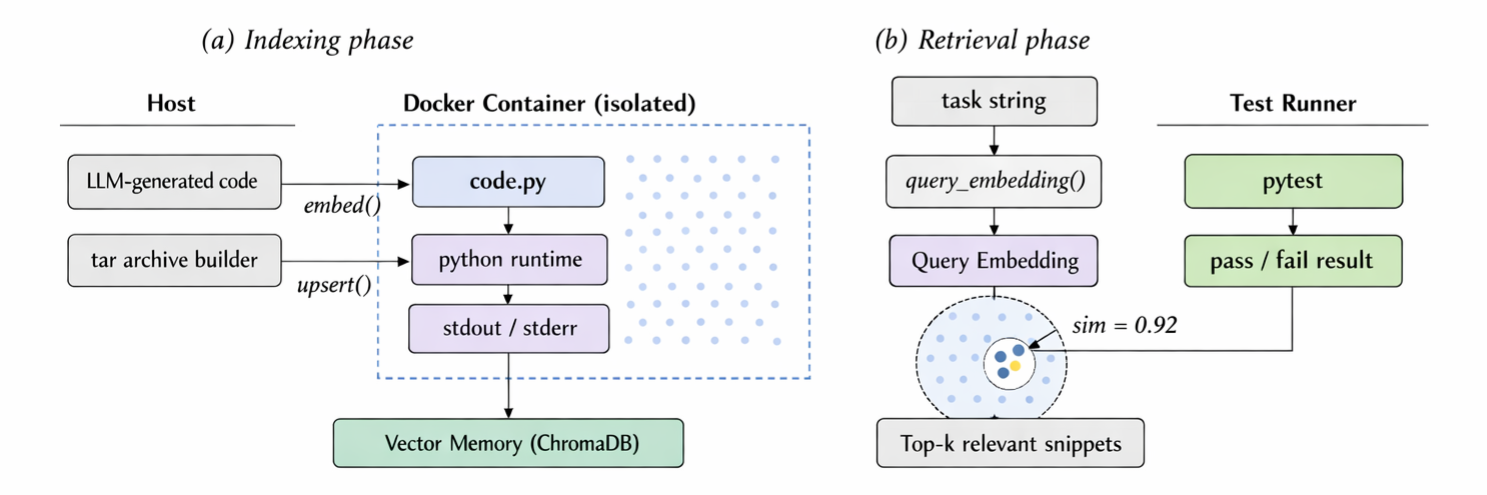
\includegraphics[width=\linewidth]{Figure4.png}
    \caption{Retrieval-Augmented Generation (RAG) architecture: (a) Offline repository indexing phase into the vector store; (b) Online semantic retrieval at inference time.}
    \label{fig:retrieval}
\end{figure}


\paragraph{Repository context.}
A background indexer (Algorithm~\ref{alg:indexer}) monitors
the repository using filesystem event hooks and maintains an
up-to-date embedding for every source file. The top-$k$
most relevant files are retrieved for each task and
prepended to the planning context. This gives the Planner
grounded knowledge of existing interfaces, reducing
hallucinated imports and incompatible function signatures.

% ------------------------------------------------------------
\subsection{Agent Definitions}
\label{sec:agents}

\paragraph{Planner ($A_\text{plan}$).}
The Planner receives the task $\mathcal{T}$, retrieved
memory context $\mathcal{M}_k$, and repository snippets,
and produces a structured execution plan:

\begin{equation}
  P = \text{LLM}(\pi_\text{plan},\;
      [\mathcal{T};\, \mathcal{M}_k;\, \mathcal{R}_k])
\end{equation}

\noindent $P$ is a JSON object containing a natural language
explanation and an ordered list of steps
$P = \{s_1, \dots, s_m\}$, where each step $s_i$ specifies
an agent assignment $s_i.\text{agent} \in \mathcal{A}$, a
description $s_i.\text{desc}$, and an optional target file
$s_i.\text{file}$.

\paragraph{Coder ($A_\text{code}$).}
For each coder step $s_i$, the Coder generates either
(a) a complete new implementation or (b) a minimal unified
diff~\cite{uniform_diff} if a target file exists:

\begin{equation}
  c_i =
  \begin{cases}
    \text{LLM}(\pi_\text{code}^\text{new},\; s_i.\text{desc})
      & \text{if } s_i.\text{file} = \emptyset \\
    \text{Apply}(\text{LLM}(\pi_\text{code}^\text{diff},\;
      [s_i.\text{desc};\, f_{s_i}]),\; f_{s_i})
      & \text{otherwise}
  \end{cases}
\end{equation}

\noindent where $f_{s_i}$ is the content of the target file
and $\text{Apply}(\cdot)$ patches the original using the
\texttt{unidiff} library. Diff-based editing preserves
unchanged lines, reducing error surface and token cost
compared to full-file regeneration.

\paragraph{Tester ($A_\text{test}$).}
Given the generated code $c_i$, the Tester produces a suite
of \texttt{pytest} test cases covering typical usage, edge
cases, and exception paths:

\begin{equation}
  \tau_i = \text{LLM}(\pi_\text{test},\;
           [c_i;\, s_i.\text{desc}])
\end{equation}

\paragraph{Debugger ($A_\text{debug}$).}
If execution of $(c_i, \tau_i)$ in the sandbox returns a
non-zero exit code or a \texttt{pytest} \texttt{FAILED}
result, the Debugger receives the code and the full error
output and produces a corrected version:

\begin{equation}
  c_i' = \text{LLM}(\pi_\text{debug},\; [c_i;\, e_i])
\end{equation}

\noindent where $e_i$ is the combined stdout/stderr from
the failed run. This loop repeats up to $N_\text{retry}$
times (default $N_\text{retry} = 3$).

\paragraph{Critic ($A_\text{crit}$).}
After all steps complete, the Critic reviews the full
result set and returns a binary verdict:

\begin{equation}
  v = \text{LLM}(\pi_\text{crit},\;
      [\mathcal{T};\, \{(s_i, c_i, e_i)\}_{i=1}^m])
      \in \{\texttt{PASS},\, \texttt{FAIL}\}
\end{equation}

\noindent A \texttt{PASS} verdict triggers persistence of
$(\mathcal{T}, \hat{c})$ into episodic memory
$\mathcal{M}$ for future retrieval.

% ------------------------------------------------------------
\subsection{Sandboxed Execution}
\label{sec:sandbox}

All generated code is executed inside a disposable Docker
container with strict resource constraints: 512\,MB memory
limit, 0.5 CPU quota, a 64-process PID cap, and networking
disabled  as shown in Figure~\ref{fig:sandbox}. Code is injected via the Docker \texttt{put\_archive}
API as an in-memory tar archive, avoiding filesystem writes
on the host. The container is force-removed after every run
regardless of outcome.


\begin{figure}[ht]
    \centering
    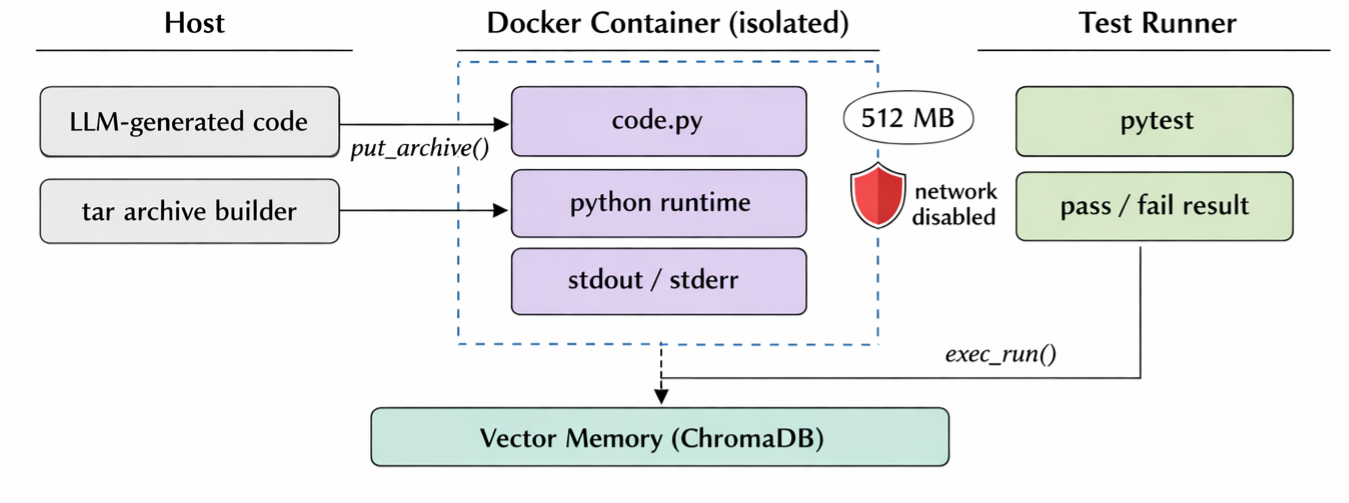
\includegraphics[width=0.85\linewidth]{Figure3.png}
    \caption{Isolated Docker sandbox execution environment. The 512\,MB memory limit and disabled networking ensure security and reproducibility.}
    \label{fig:sandbox}
\end{figure}

Formally, let $\text{Sandbox}(c, \tau)$ return
$(o, e) \in \Sigma^* \times \Sigma^*$ where $o$ is stdout
and $e$ is stderr. Execution is considered successful iff:

\begin{equation}
  \text{pass}(c, \tau) =
  \mathbf{1}[e = \emptyset \;\wedge\;
  \texttt{FAILED} \notin o \;\wedge\;
  \texttt{ERROR} \notin o]
\end{equation}

% ------------------------------------------------------------
\subsection{Full Orchestration Algorithm}
\label{sec:algorithm}

Algorithm~\ref{alg:main} summarizes the complete pipeline.

\begin{algorithm}[t]
\caption{AgentForge Orchestration}
\label{alg:main}
\begin{algorithmic}[1]
\REQUIRE Task $\mathcal{T}$, context files $\mathcal{F}$,
         memory $\mathcal{M}$, repo index $\mathcal{R}$
\ENSURE  Verified code $\hat{c}$ or \textsc{Fail}

\STATE $\mathcal{M}_k \leftarrow \text{Retrieve}(\mathcal{T}, \mathcal{M})$
\STATE $\mathcal{R}_k \leftarrow \text{Retrieve}(\mathcal{T}, \mathcal{R})$
\STATE $P \leftarrow A_\text{plan}(\mathcal{T}, \mathcal{M}_k, \mathcal{R}_k)$
\STATE $\hat{c} \leftarrow \emptyset$,\; results $\leftarrow []$

\FOR{each step $s_i \in P.\text{steps}$}
  \IF{$s_i.\text{agent} = \texttt{coder}$}
    \STATE $\hat{c} \leftarrow A_\text{code}(s_i, \mathcal{F}, \text{results})$
    \STATE results.append$(\hat{c})$

  \ELSIF{$s_i.\text{agent} = \texttt{tester}$}
    \STATE $\tau \leftarrow A_\text{test}(\hat{c}, s_i)$
    \STATE $(o, e) \leftarrow \text{Sandbox}(\hat{c}, \tau)$
    \STATE $n \leftarrow 0$
    \WHILE{$\neg\text{pass}(\hat{c}, \tau)$ \AND $n < N_\text{retry}$}
      \STATE $\hat{c} \leftarrow A_\text{debug}(\hat{c}, e)$
      \STATE $(o, e) \leftarrow \text{Sandbox}(\hat{c}, \tau)$
      \STATE $n \leftarrow n + 1$
    \ENDWHILE
    \STATE results.append$(o, e)$

  \ELSIF{$s_i.\text{agent} = \texttt{critic}$}
    \STATE $v \leftarrow A_\text{crit}(\mathcal{T}, \text{results})$
    \STATE results.append$(v)$
  \ENDIF
\ENDFOR

\STATE $v_\text{final} \leftarrow A_\text{crit}(\mathcal{T}, \text{results})$
\IF{$v_\text{final} = \texttt{PASS}$}
  \STATE $\mathcal{M}.\text{store}(\mathcal{T}, \hat{c})$
  \RETURN $\hat{c}$
\ELSE
  \RETURN \textsc{Fail}
\ENDIF
\end{algorithmic}
\end{algorithm}

% ------------------------------------------------------------
\subsection{Streaming Output}
\label{sec:streaming}

To support interactive use, the Orchestrator exposes a
streaming interface over Server-Sent Events (SSE) and
WebSocket. Each token produced by the Coder agent is
forwarded to the client as it arrives, using Python
async generators and FastAPI's \texttt{EventSourceResponse}.
This enables real-time inspection of the generation process
without waiting for pipeline completion.

% ------------------------------------------------------------
\subsection{Complexity Analysis}
\label{sec:complexity}

Let $L$ be the average prompt length in tokens and $G$ the
average generated length. A single pipeline run incurs
$O(|\mathcal{A}| \cdot (L + G))$ tokens in the non-debug
case, and $O(|\mathcal{A}| \cdot (L + G) \cdot N_\text{retry})$
in the worst case. Retrieval adds $O(d \log n)$ per query
for a HNSW index of $n$ embeddings in $d$ dimensions. All
agent calls are embarrassingly parallelizable within a plan
step when step dependencies permit.
